\begin{frame}{Qu'est-ce qu'un système distribué ?}

    \begin{columns}[onlytextwidth]% align columns
        \begin{column}{.65\textwidth}
            \begin{definitionbox}
                Un système distribué est un ensemble de \textbf{machines
                indépendantes} qui sont \textbf{interconnectées} qui
                apparaissent aux yeux de l'utilisateur comme un système unique
                et cohérent, tout en \textbf{communiquant ensemble} via le
                réseau.
            \end{definitionbox}
        \end{column}%
        \hfill%
        \begin{column}{.4\textwidth}
            \begin{figure}[htb]
                \centering
                \resizebox{0.8\textwidth}{!}{
                    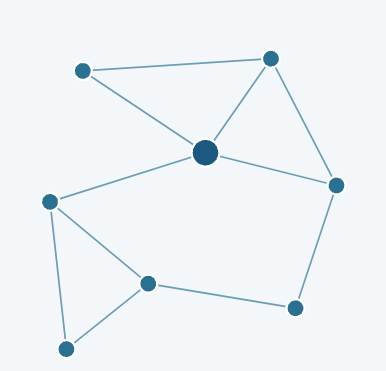
\includegraphics[width=\textwidth]{img/distributed-system.png}
                }
            \end{figure}
        \end{column}%
    \end{columns}

\end{frame}

\begin{frame}{Pourquoi distribuer ?}

    \begin{itemize}
        \item \textbf{Scalabilité} : répartir la charge sur plusieurs machines
              pour dépasser les limites d'une seule
        \item \textbf{Disponibilité} : tolérer la panne d'un nœud sans arrêter
              le service
        \item \textbf{Latence} : rapprocher les données/calculs des utilisateurs
              géographiquement
        \item \textbf{Coût} : utiliser du matériel standard plutôt qu'une
              machine surpuissante unique
    \end{itemize}
\end{frame}
